Para a implementação da arquitetura, a solução em \emph{cloud}~\cite{heroku} foi utilizada. Ela oferece infra-estrutura como serviço de hospedagem, possibilitando desenvolvimento em \emph{Ruby on Rails}. %Dentre estas alternativas, a implementação foi realizada em \emph{Ruby on Rails} (RoR), por maior experiência de membros do grupo e pela versatilidade da linguagem, que se mostra mais direta para a implementação, embora qualquer outro \emph{framework} e linguagem pudessem ser utilizados.
%
%
A arquitetura do \emph{framework}~\cite{ror} é completamente baseada no paradigma \emph{Model View Controler} (MVC), facilitando a organização dos módulos de nosso mecanismo. Desta forma, a estrutura do código escrito em RoR é composta de componentes de Modelo, de Visão e de Controle. Componentes de \textbf{modelo} correspondem aos dados - como eles são armazenados, obtidos, correlacionados. A parte de \textbf{visão} corresponde à parte gráfica da aplicação. Finalmente, \textbf{controladores} realizam a manipulação de dados como um todo, e correspondem à parte lógica e funcional do código. Eles funcionam também como uma ponte entre modelo e visão, para que os dados transitem em ambos os sentidos.
%
% Como \emph{framework}, foi utilizado o Ruby on Rails (RoR),  por ser baseado no paradigma \emph{Model View Controler}, que facilita a divisão necessária para os módulos da arquitetura. 

Considerando o RoR, o submódulo analizador de tráfego (AT) da arquitetura corresponde a um controlador. Uma requisição à aplicação será interceptada por esse componente de controle, que realizará a medição de estatísticas, e imediatamente acionará o controlador que corresponde ao funcionamento da aplicação em si. Deve-se notar, contudo, que o tempo despendido neste controlador é ínfimo. Em outras implementações, caso se perceba que o tempo afete o funcionamento do mecanismo de mitigação, este processamento poderia ainda ser realizado em segundo plano.

Caso o AT detecte a existência de um possível ataque, uma nova instância \emph{cloud} é criada pelo submódulo INA e a aplicação é replicada para esta instância, paralisando a aplicação original, que passa a responder apenas como redirecionador. O processo de reinstanciação da aplicação na implementação realizada consiste da existência prévia de uma segunda aplicação, inicialmente sem nenhum recurso alocado. %Entretanto, embora esta instância estaria pronta para que seus processos sejam escalados assim que necessário, esta abordagem não se comporta adequadamente no cenário de reinstanciação recursiva. A segunda abordagem envolve a hospedagem do projeto em um repositório do GitHub, que poderá ser clonado para a especificação da segunda instância a partir do código Ruby. 

Uma particularidade interessante do \emph{framework} RoR é a existência de um arquivo de rotas. A implementação do submódulo redirecionador de tráfego (RT) é realizada em cima deste arquivo, chamado \emph{routes.rb}. Para a exibição de qualquer página dinâmica da aplicação, o arquivo de rotas é inevitavelmente chamado. Desta forma, ele é utilizado para a adição de clientes na \emph{blacklist} e respectiva filtragem dos clientes bloqueados pelo gerenciador da \emph{blacklist} (GB). No redirecionamento do tráfego para uma nova instância, uma entrada será adicionada, bloqueando o cliente em questão por determinado tempo.

% \begin{figure}[ht!]
% 	\centering
% 	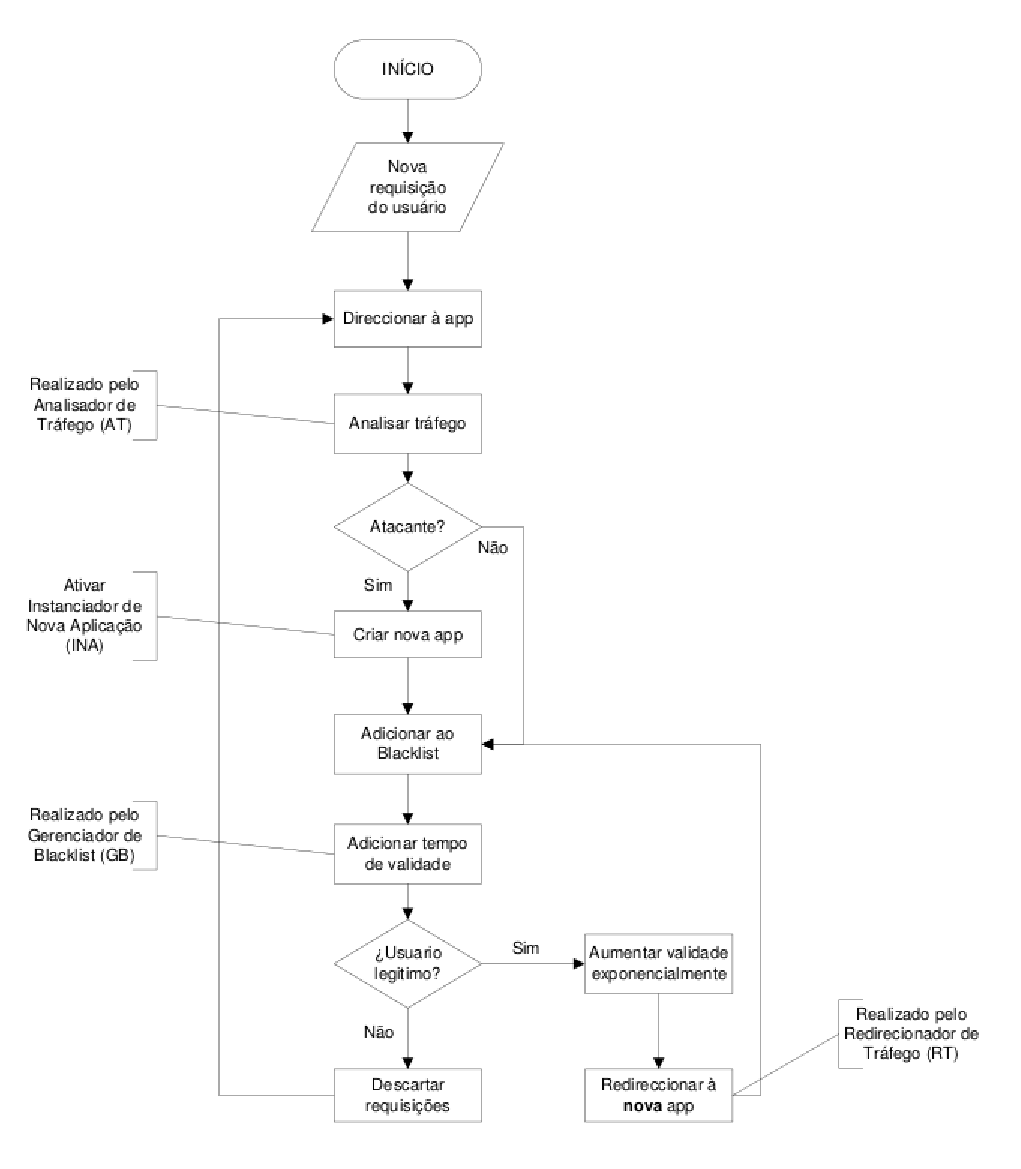
\includegraphics[width=0.55\textwidth]{images/dfd.eps}
% 	\hskip 1cm
% 	\caption{Funções da arquitetura de mitigação de DDoS}
% 	\label{fig:dfd}
% \end{figure}

A \emph{blacklist} em si e as diversas outras variáveis de controle são gerenciadas pela base de dados em \emph{cloud}~\cite{redis}. Esta base de dados é conhecida por sua simplicidade e eficiência. Ela basicamente mapeia \textbf{chave} e \textbf{dado}, oferecendo tempos de escrita e de leitura correspondentes à \emph{hashing}. A implementação da \emph{blacklist} foi feita utilizando o endereço IP de um cliente como chave, e o tempo que este cliente permanecerá bloqueado como dado. Por ser, indiretamente, um mecanismo de \emph{hashing}, o tempo de busca por um cliente será O(1), o que é excelente para um mecanismo que vai filtrar todo tráfego que chega à aplicação. %Uma visão estruturada das funções realizadas pela arquitetura proposta é descrita no diagrama de fluxo ilustrado na Figura~\ref{fig:dfd}.

%Por fim, um aspecto interessante do uso do Heroku são os diversos \emph{addons} já customizados para o uso nele. Em particular, existe um \emph{addon} chamado \emph{New Relic} que é designado à coleta de diversas métricas para a análise de desempenho. Com seu uso, será possível saber com precisão o que se passa em todas as instâncias \emph{cloud} de uma perspectiva diretamente interna à esta \emph{cloud}. Assim, poderemos coletar dados não só da perspectiva externa à \emph{cloud}, perspectiva de usuário, como também, de perspectiva interna~à~ela.